\documentclass{article}
\usepackage{graphicx}
\usepackage[utf8]{inputenc}
\usepackage[hidelinks]{hyperref}
\usepackage{caption}
\usepackage{verbatim}

\renewcommand*\contentsname{Índice}

\begin{document}

\begin{figure}[!htb]
\minipage{0.32\textwidth}
	\includegraphics[width=\linewidth]{"../../../../LogoSEP".png}
\endminipage\hfill
\minipage{0.32\textwidth}
	\includegraphics[width=\linewidth]{"../../../../LogoTecnologicoNacionalMexico".PNG}
\endminipage\hfill
\minipage{0.32\textwidth}
	\includegraphics[width=\linewidth]{"../../../../LogoITT".png}
\endminipage\hfill
\end{figure}

\begingroup
\LARGE
\begin{verbatim}
Subdirección Académica
Departamento de Sistemas y Computación
Ingeniería en Sistemas Computacionales
Semestre: Enero - Junio 2017
Materia: Sistemas Programables (3SC8A)

Propuesta de proyecto
Catafixia moderna

Integrantes:
Salcedo Morales José Manuel (13211419)
Espinoza Covarrubias Silverio Alejandro (13211465)
Alvarez Corral Miguel Angel (13211384)

Nombre del catedrático:
Ingeniero Luís Alberto Mitre Padilla

Fecha de entrega:
Tijuana, Baja California a 30 de Marzo de 2017
\end{verbatim}
\endgroup

\newpage
\tableofcontents

\newpage
\section{Introducción}
Extra\~nando a Chabelo? Todos lo hacemos. Por ello, se emulara el concurso de la catafixia con una ligera configuracion.
\newline En este, hay tres botones para las tres catafixias. Hay un boton para cada una.
\newline Hay un sensor en cada catafixia con un valor mostrado en un display distinto.
El jugador tiene que encontrar el sensor que se le pida con el poder del se\~nor director. Perdiendo si es el que encuentra primero.

\section{Sensores}
\begin{itemize}
	\item Boton
	\item Fotoresistencia
	\item Temperatura y humedad
	\item Sensor de sonido
\end{itemize}

\newpage
\section{Interfaz Grafica}
\textbf{Web}
\newline Uso de javascript puro (con HTML obviamente), en conjunto con otro lenguaje de programacion para el control de los contenidos e informacion general de las catafixias y el estado del jugador.
\newline El usuario de la pagina tiene el control de hechar a perder la lectura de un sensor o inclusive cambiar el valor de muestreo para el usuario de un sensor.

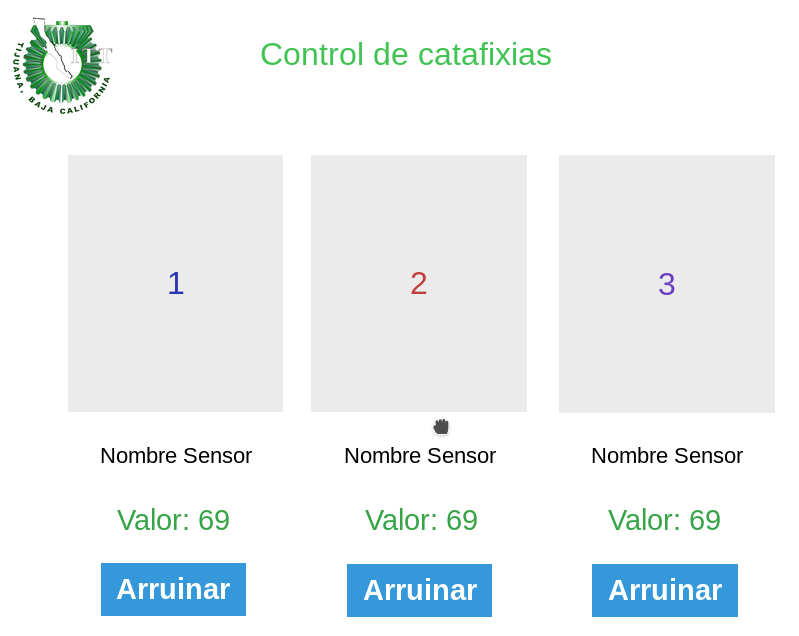
\includegraphics[width=\linewidth]{Bosquejo}


\end{document}